\documentclass[13pt]{article}
\usepackage[margin=1in]{geometry}
\usepackage{fancyhdr}
\usepackage[noindentafter]{titlesec}
\usepackage[T1]{fontenc}
\usepackage[scaled]{helvet}
\usepackage[pdftex]{graphicx}
\usepackage{hyperref}
\usepackage{multicol}
\usepackage{tocloft}
\usepackage{etoc}
\usepackage{float} 
\usepackage{subfiles}
\usepackage{framed}
\usepackage{fancybox}
\usepackage{multirow}
\usepackage{tabularx}
\usepackage{threeparttable}
\usepackage{caption}
\usepackage{longtable}
\usepackage{pifont}

\graphicspath{{Images//}}
% set fond
\renewcommand*\familydefault{\sfdefault}
\sffamily

\pagestyle{fancy}
\renewcommand{\footrulewidth}{0.4pt}
% define page header/footer
\lhead{}
\chead{}
\rhead{Space Shuttle Ultra Manual}
\lfoot{}
\cfoot{\thepage}
%\rfoot{\leftmark\\ \rightmark}

%\titleformat*{\subsection}{\bfseries\center}
\titleformat{\paragraph}[hang]{\bfseries}{\theparagraph}{1em}{}
%\newcommand{\paragraphbreak}{\vspace{1em}}

\newcommand{\NOTE}[1]{
  \begin{center}
    \textbf{NOTE} \\
    {#1}
  \end{center}}
\newcommand{\CAUTION}[1]{
  \begin{framed}
    \begin{center}
      \textbf{CAUTION} \\
    \end{center}
    {#1}
  \end{framed}
}
\newcommand{\WARNING}[1]{
  \doublebox{
    \begin{minipage}{0.934\linewidth}
      \begin{center}
        \textbf{WARNING} \\
      \end{center}
      {#1}
    \end{minipage}
  }
}


\begin{document}
%\dosecttoc
%\pagenumbering{roman}
\begin{titlepage}

\begin{center}

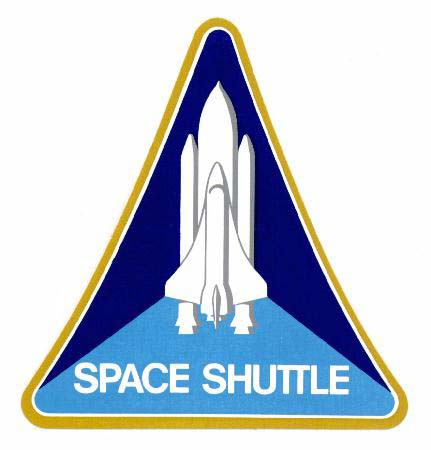
\includegraphics[width=0.35\textwidth]{SSP.jpg}\\[1cm]

\textsc{\LARGE Space Shuttle Ultra}\\[1.5cm]

\textsc{\Large Version 4.2}\\[0.5cm]

\huge \bfseries SSU Operations Manual\\[0.4cm]

\vfill

{\large \today}

\end{center}
\end{titlepage}


\newpage
\thispagestyle{empty}
\vspace*{\fill}
\begin{quote}
\centering
\textit{The Space Shuttle had a 30 year run like none other. Four times I was blessed with the opportunity to travel to space aboard this marvelous spacecraft. There has never been a vehicle quite like it$\colon$ a reusable spacecraft, with the beauty of an airplane, the capacity to carry eight astronauts to space and a 60-foot payload bay. The Shuttle's three-decade long run was nothing short of remarkable.}
\end{quote}
\begin{flushright}
Charles F. Bolden Jr. - NASA Administrator, 2015
\end{flushright}
\vspace*{\fill}
\newpage


\pagenumbering{roman}

\section*{PREFACE}
\begin{multicols*}{2}
%\addcontentsline{toc}{section}{PREFACE}
Space Shuttle Ultra (SSU) is an addon for Orbiter Space Flight Simulator.  The purpose of this addon is to fully simulate the NASA's Space Transportation System Program.  Currently only a few elements have been completed and work on others is ongoing.\\
\\
The basis for this addon was the Space Shuttle Deluxe but through adding additional subsystems and taking full advantage of the 2010 version of Orbiter, the current SSU has few similarities to the original Deluxe.  Currently, SSU simulates a number of systems, displays, and procedures of the real shuttle and can be used along with real NASA Flight Data File (FDF) checklists to complete tasks.  These checklists can be found at the \href{http://www.nasa.gov/centers/johnson/news/flightdatafiles/index.html}{NASA Flight Data Files} web page (\url{http://www.nasa.gov/centers/johnson/news/flightdatafiles/index.html}), and provide a good reference for other procedures. The NASA Flight Data Files site includes checklists for all missions after STS-107, as well as generic checklists. \\
\\
Additional documentation containing background information about the shuttle and its systems can be found \href{http://sourceforge.net/projects/shuttleultra/files/References/}{here} (\url{http://sourceforge.net/projects/shuttleultra/files/References/}).\\
\\
Other good NASA references are the Shuttle Crew Operations Manual (SCOM), the DPS Dictionary, and the various Workbooks and Handbooks that are available on the Internet (these can also be found at the above link). \\
\\
This document contains the condensed material taken from various NASA documents as well and Orbiter and SSU specific information.  The goal of this document is to provide a typical Orbiter User the information need to perform basic SSU flights as well as  to aid in basic custom mission creation.  Separate documents will be provided for developers who would like to create a SSU compatible payloads and scenarios.\\
\\
This document is formatted to look the same as the SCOM to facilitate changing from one document to the other.  Additional information or clarification is presented in three formats: notes, cautions, and warnings. Notes provide amplifying information of a general nature. Cautions provide information and instructions necessary to prevent hardware damage or malfunction (not yet simulated). Warnings provide information and instructions necessary to ensure crew safety (also not simulated). The formats in which this material appears are illustrated below.\\
\NOTE{A barberpole APU/HYD READY TO START talkback will not inhibit a start.}
\CAUTION{After an APU auto shutdown, the APU FUEL TK VLV switch must be taken to CLOSE prior to inhibiting auto shutdown logic. Failure to do so can allow the fuel tank isolation valves to reopen and flow fuel to an APU gas generator bed that is above the temperature limits for safe restart.}
\WARNING{The FUEL CELL REAC switches on panel R1 are in a vertical column with FUEL CELL 1 REAC on top, FUEL CELL 3 REAC in the middle, and FUEL CELL 2 REAC on the bottom. This was done to allow the schematic to be placed on the panel. Because the switches are not in numerical order, it is possible to inadvertently close the wrong fuel cell reactant valve when shutting down a fuel cell.}
\end{multicols*}

\newpage
\tableofcontents
\newpage

\pagenumbering{arabic}
\section{INSTALLATION INSTRUCTIONS}
\begin{multicols*}{2}
\noindent
SSU requires the following addons to be installed:
\begin{enumerate}
\item OrbiterSound 4.0 (\url{http://orbiter.dansteph.com/index.php?disp=d})
\item KSC hires tiles (\url{http://www.orbithangar.com/searchid.php?ID=5583})
\item Vandenberg AFB (\url{http://www.orbithangar.com/searchid.php?ID=2380})
\end{enumerate}
CRT MFD needs to be enabled (Orbiter Launchpad $\rightarrow$ Modules $\rightarrow$ check \textit{CRT} box).\\
The following lines need to be added to the list of textures of the ''<orbiter\_installation>\textbackslash Config\textbackslash Base.cfg'' file$\colon$\\
$\rightarrow$ NOR1735tex\\
$\rightarrow$ NOR2305tex\\
Using the D3D9 graphics client is strongly recommended (although not required). The \textit{Enable geometry instancing} option in the D3D9 Advanced Setup dialog (Orbiter Launchpad $\rightarrow$ Video $\rightarrow$ Advanced) should be unchecked.\\
If you encounter the error ''msvcp120.dll is missing'' you need to download the Microsoft Visual C++ Redistributable for Visual Studio 2013.\\
\\
\noindent
\WARNING{The SSU installation overwrites the default Earth.cfg file.}
\end{multicols*}

\newpage
\section{GENERAL DESCRIPTION}
\begin{multicols*}{2}
%\secttoc
\renewcommand{\cfttoctitlefont}{\bf}
\localtableofcontents
%\begin{tabular}{|p{6.9cm}  p{0.25cm}|}
%	\hline
%	&\\[0.1cm]
%	CONTENTS & \\[0.4cm]
%	1.1	OVERVIEW & 2\\
%	1.2	ORBITER AND SSU & 7\\
%	1.3	COMPONENTS OVERVIEW & 10\\
%	\hline
%\end{tabular}
%\\[0.4cm]
\noindent
\\
The section provides general background information about the orbiter, its configuration and coordinate system, the nominal mission profile, and general procedures followed during a shuttle mission.
\\
Also included in this section is keyboard commands for SSU but will not include standard Orbiter keyboard commands. See Orbiter.pdf for standard Orbiter keyboard commands.
\end{multicols*}

\subsection{Overview}
\begin{multicols*}{2}
\renewcommand{\cfttoctitlefont}{\bf}
\localtableofcontents
%\begin{tabular}{|p{6.9cm} p{0.25cm}|}
%	\hline
%	&\\[0.1cm]
%	CONTENTS & \\[0.4cm]
%	Space Shuttle Overview & 2\\
%	Nominal Mission Profile & 2\\
%	Launch and Landing Sites & 4 \\
%	Shuttle Location Codes &  4\\
%	\hline
%\end{tabular}

\subsubsection{Nominal Mission Profile}
%\addcontentsline{toc}{subsection}{Nominal Mission Profile}
SSU has reached a point of development that almost a full mission profile can be simulated.

\paragraph{Launch}
The launch is controlled by autopilot. The autopilot targets a set of desired parameters defined in the mission file (altitude, velocity and inclination) at main engine cutoff (MECO).
After MECO, the ET is jettisoned and the +Z RCS thrusters are automatically fired to translate the orbiter away from the ET. \\
\\
Procedures for this phase of the mission can be found in the NASA Ascent Checklist.
\paragraph{Orbit Insertion and Circularization}
The nominal ascent profile, referred to as "direct insertion," places the vehicle in a temporary elliptical orbit at MECO, with the perigee in the Earth's atmosphere. Orbital altitudes can very depending on mission requirements. The crew performs an OMS burn, designated as ``OMS 2'', to stabilize the orbit. This burn can add anywhere between 200 to 550 fps to the vehicle's orbital velocity, as necessary.\\
%\\
%In cases of severe performance problems during the ascent, the vehicle may find itself well short of the expected MECO velocity, and even suborbital. In such cases, the crew performs what is call an ``OMS 1'' burn shortly after MECO, which raises the orbit to a safe altitude. They then perform an OMS 2 burn to stabilize that orbit.\\
\\
When simulating early missions with SSU, the orbiter will perform what was known as a ``standard insertion''. This will place the orbiter in a heads down suborbital orbit at MECO and will require an OMS 1 burn to raise the apogee, followed by an OMS 2 burn.  This ascent profile was used for the first ten missions, STS-1 though STS-41B.\\
\\
After ET separation (and before the OMS 2 burn), the ET umbilical doors are closed.\\
\\
Procedures for this phase of the mission can be found in the NASA Ascent Checklist.
\paragraph{Orbit}
On orbit, the forward and aft RCS jets provide attitude control of the orbiter, as well as any minor translation maneuvers along a given axis. The OMS engines are used to perform orbital transfers, such as those done to rendezvous with the International Space Station (ISS). Mission objectives while in orbit has ranged from ISS assembly and logistics, payload deployment and retrieval, to scientific experiments. Also several planned, but not flown, missions are able be simulated with SSU including Shuttle-Centaur flights and Vandenberg missions.
\\
The procedures needed on orbit differ significantly based on the mission objectives. Checklists for STS-114 and subsequent missions can be found at the Flight Data Files page. The Orbit Operations Checklist, Orbit Pocket Checklist and PDRS Operations Checklist (all available at the Flight Data Files page) contain generic information for operations that are frequently performed (i.e. OMS burns).\\
\\
During the last full day on-orbit (the day before the planned deorbit burn), the FCS checkout and RCS hotfire tests are performed. Procedures for these tests can be found in the Orbit Operations Checklist.
\paragraph{Deorbit}
At the completion of orbital operations, the RCS is used to orient the orbiter in a tail-first attitude. The two OMS engines are burned to lower the orbit such that the vehicle enters the atmosphere at a specific altitude and range from the landing site. The deorbit burn usually decreases the vehicle's orbital velocity anywhere from 200 to 550 fps, depending on orbital altitude.  When the deorbit burn is complete, the RCS is used to rotate the orbiter's nose forward for entry. The RCS jets are used for attitude control until atmospheric density is sufficient for the pitch, roll, and yaw aerodynamic control surfaces to become effective. \\
\\
Procedures for deorbit prep and the deorbit burn are in the Deorbit Prep Checklist and the Entry Checklist. Mission-specific details are in the Entry Flight Supplement.
\paragraph{Entry}
In real life, reentry is normally controlled automatically by the Aerojet Digital Autopilot (DAP) from entry interface (EI) through Terminal Area Energy Management (TAEM), to $\sim$ Mach 1, where the CDR takes control of the orbiter. SSU has a fully functioning entry autopilot which provides guidance and control from EI to 2000 ft (the start of the preflare). It is also possible to fly the shuttle manually. The speedbrake is usually controlled automatically throughout entry, but can be controlled manually. See Section \ref{sec:entry} for more details.
The Heads-Up Display (HUD) becomes active at Mach 2.5. Guidance commands are displayed on the HUD from Mach 2.5 until the start of the final flare phase. \\
\\
The landing gear are automatically armed at 2000 ft and deployed at 300 ft. In real life, this is done manually by the PLT. \\
\\
Procedures for entry and found in the Entry Checklist. Mission-specific details are in the Entry Flight Supplement.
\vfill
\subsubsection{Shuttle Coordinate Frame}
\begin{figure}[H]
  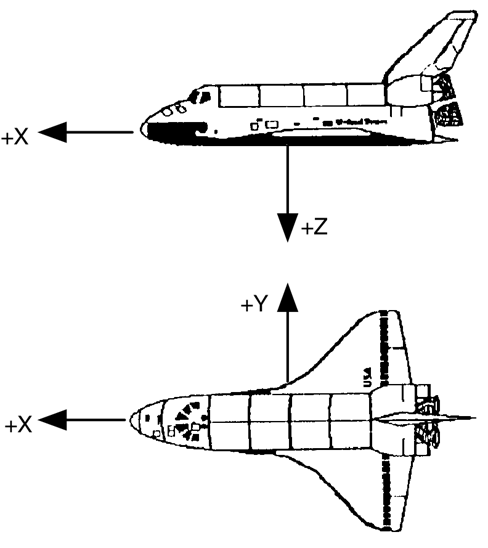
\includegraphics[width=0.5\textwidth]{ShuttleBodyAxisSystem.png}
  \caption{Body Axis Coordinate System (image from SCOM)}
  \label{fig:BodyAxisSystem}
\end{figure}
Figure \ref{fig:BodyAxisSystem} shows the shuttle Body Axis Coordinate system. This coordinate system is used in the NASA documents and checklists, as well as this manual.
It should be noted that the Body Axis Coordinate frame is different from the normal Orbitersim frame.

\subsubsection{Shuttle Location Codes}
%\addcontentsline{toc}{subsection}{Shuttle Location Codes}
Orbiter location codes enable crewmembers to locate displays and controls, stowage compartments and lockers, access panels, and wall-mounted equipment in the orbiter crew compartments. The crew compartments are the flight deck, middeck, and airlock. Because of compartment functions and geometry, each has a unique location coding format.
\\
Currently SSU only simulates the flight deck panels. Eventually panels in the middeck will be simulated and at that time the middeck location coding will be included in this manual.
\\
A flight deck location code consists of two or three alphanumeric characters. The first character is the first letter of a flight deck surface as addressed while sitting in the commander/pilot seats.
The second and third characters are numbers identifying the relative location of components on each flight deck surface. Table \ref{tab:PanelNumbering} lists the surfaces and the numbering philosophy for each surface.
Figures \ref{fig:FlightDeckLocCodes1} and \ref{fig:FlightDeckLocCodes2} show the flight deck panels and their location codes.
\begin{table}[H]
  \begin{tabularx}{\linewidth}{l | X}
    SURFACES & NUMBERING PHILOSOPHY \\
    \hline
    L - Left & \multirow{3}{\linewidth}{Numbered from top to bottom, forward to aft} \\
    R - Right & \\
    C - Center Console & \\
    \hline
    O - Overhead & Numbered from left to right, forward to aft \\
    \hline
    F - Forward & \multirow{2}{\linewidth}{Numbered left to right, top to bottom (facing the surface)} \\
    A - Aft & \\
    \hline
    \multirow{3}{*}{W - Windows} & \textbf{Forward} (W1 through W6): numbered left to right facing forward \\
    & \textbf{Overhead} (W7 \& W8): numbered left to right facing aft \\
    & \textbf{Aft} (W9 \& W10): numbered left to right facing aft \\
    \hline
    S - Seats & CDR seat is S1 and PLT seat is S2
  \end{tabularx}
  \caption{Flight Deck Numbering scheme}
  \label{tab:PanelNumbering}
\end{table}
%\\
%\end{multicols}
%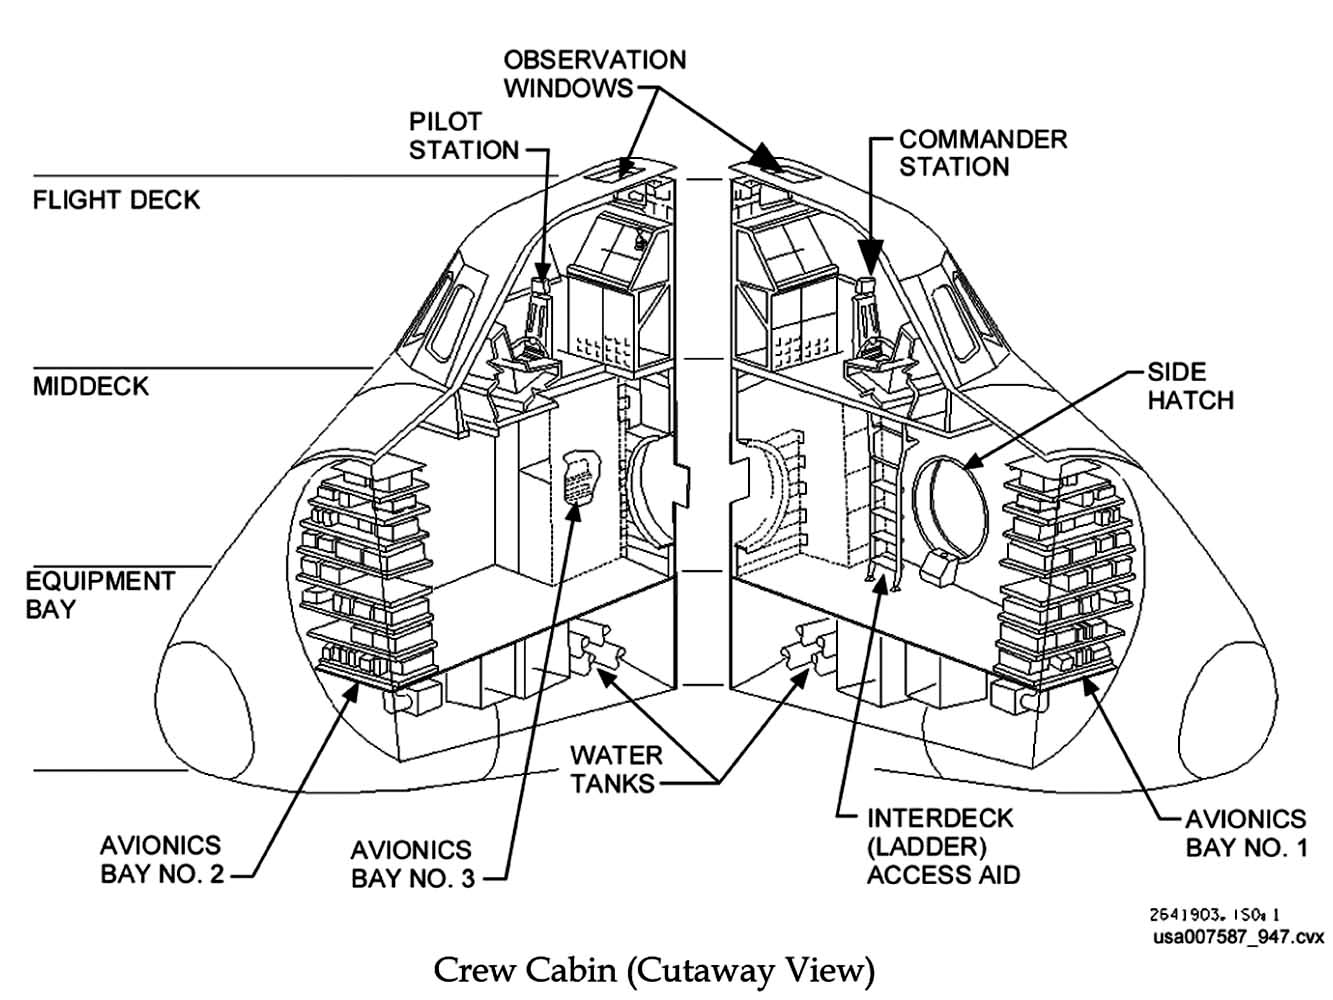
\includegraphics[width=0.85\textwidth]{Crew Cabin (Cutaway).jpg}
%\begin{multicols}{2}
%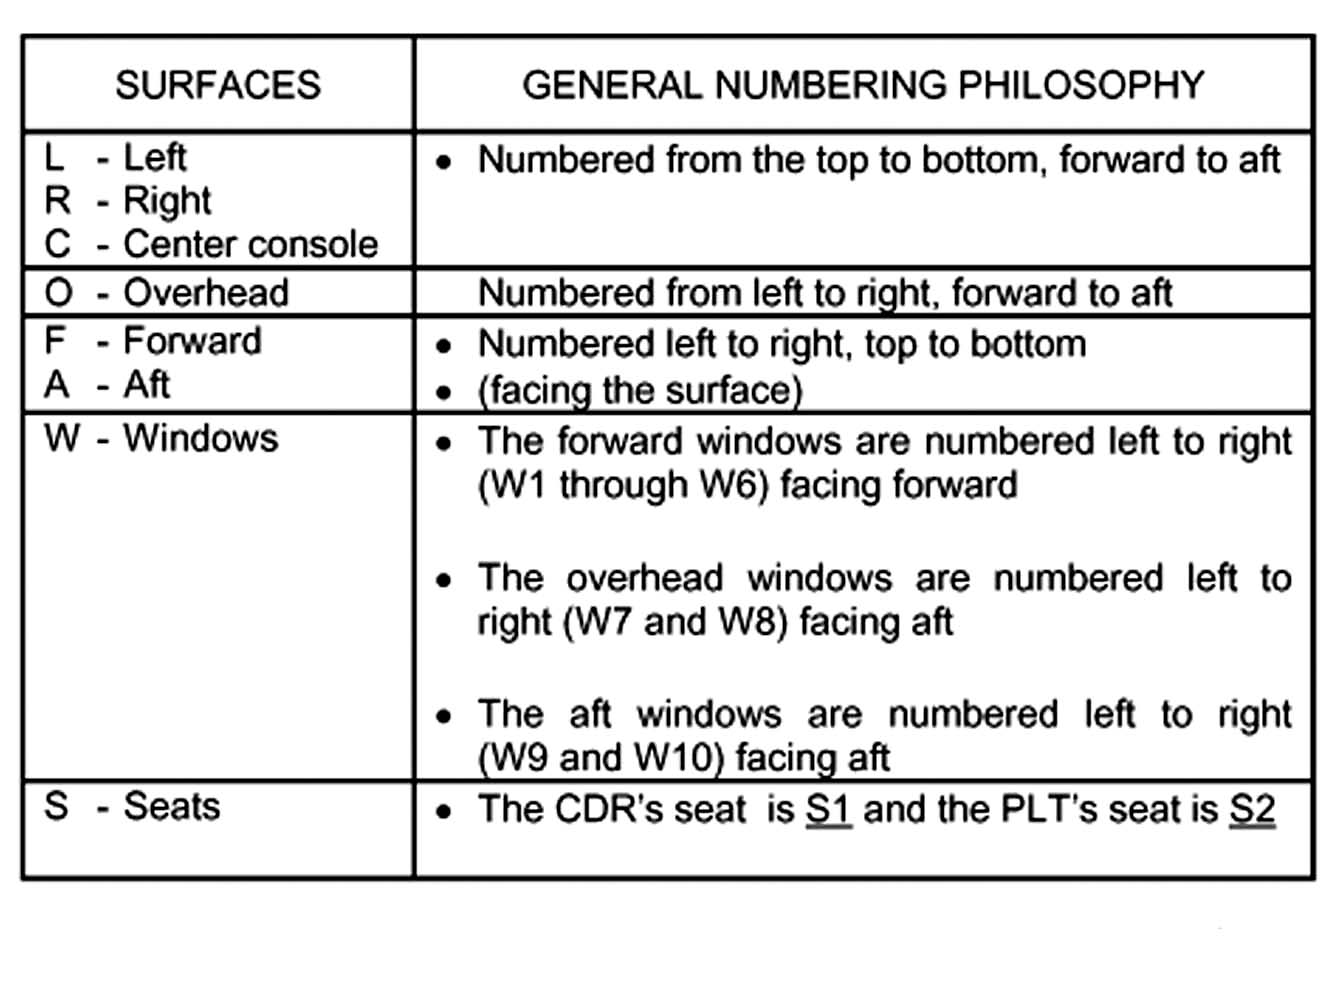
\includegraphics[width=0.5\textwidth]{FD_Codes_Chart.jpg}
\end{multicols*}

\newpage
\begin{figure}[H]
  \centering
  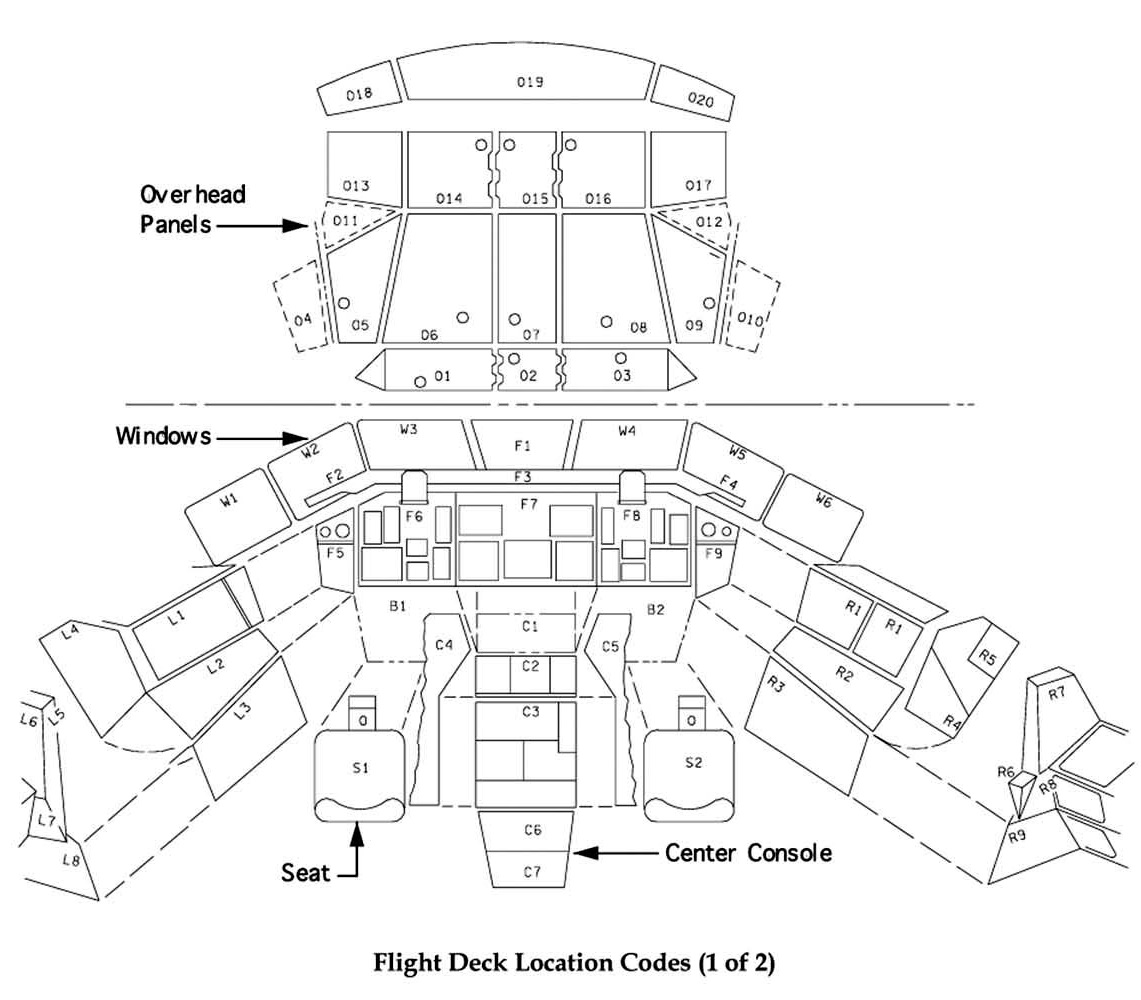
\includegraphics[width=\textwidth,height=0.5\textheight,keepaspectratio]{Flight_Deck_Loc_Codes_1.jpg}
  \caption{}
  \label{fig:FlightDeckLocCodes1}
\end{figure}
\begin{figure}[H]
  \centering
  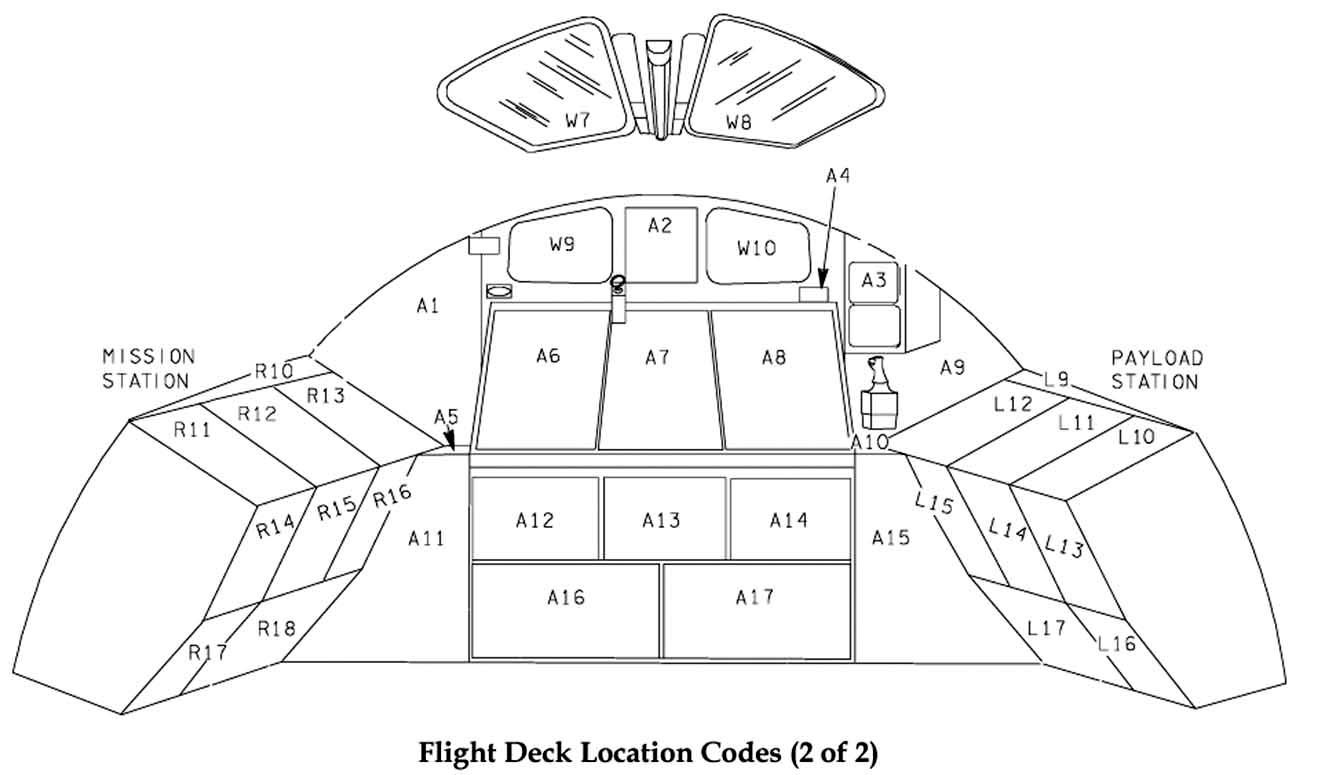
\includegraphics[width=\textwidth,height=0.35\textheight,keepaspectratio]{Flight_Deck_Loc_Codes_2.jpg}
  \caption{}
  \label{fig:FlightDeckLocCodes2}
\end{figure}

\newpage
\subsection{Orbiter and SSU}
\renewcommand{\cfttoctitlefont}{\bf}
\localtableofcontents
%\begin{tabular}{|p{7cm} p{0.25cm}|}
%	\hline
%	&\\[0.1cm]
%	CONTENTS & \\[0.4cm]
%	SSU Keyboard Commands & 7\\
%	Camera Views & 8\\
%	Payload Operations Overview & 9\\
%	\hline
%\end{tabular}


\subsubsection{SSU Keyboard Commands}
%\addcontentsline{toc}{subsection}{SSU Keyboard Commands}
The ultimate goal of SSU is to provide a complete simulation of the Space Shuttle.  This means that most of the input is done with in-simulation controls (i.e. cockpit switches, GNC keyboards, and dialog windows). This results in very few keyboard commands to operate the shuttle.

\begin{center}
  \textbf{General}\\
  Ctrl+A - toggle between controlling RCS thrusters and RMS motion\\
  Ctrl+G - arm landing gear\\
  G - deploy landing gear\\
  comma - open speedbrake by 5 percent\\
  period - close speedbrake by 5 percent\\
  \vspace{\baselineskip}

  \textbf{Alternate Translation Commands (valid only if RCS is in Rot mode)}\\
  Left/Right Arrow - left/right translation (equivalent to 1/3 on Numpad)\\
  Up/Down Arrow - up/down translation (equivalent to 8/2 on Numpad)\\
  Insert/Delete - forward/aft translation (equivalent to 9/6 on Numpad)\\
  \vspace{\baselineskip}

  \textbf{RMS}\\
  Ctrl+Enter - grapple\\
  Ctrl+Backspace - release\\
  Ctrl+O - toggle between Coarse and and Vern rates\\
\end{center}

\begin{multicols*}{2}
\subsubsection{RHC/THC}
The regular Orbitersim thruster control commands (either keyboard or joystick) are used to simulate the RHC \& THC. When controlling the RCS thrusters, the appropriate \textit{FLT CNTLR PWR} switch must be on for RHC/THC inputs to be used. There are no such restrictions when controlling the RMS (although the RMS needs to be powered on before it can move).
\\
\\
The RHCs on the real shuttle have a "soft stop" and a "hard stop" (the mechanical limit of movement). Moving the RHC out of detent (up to the soft stop) will command either a constant rotation rate or a pulse of RCS firings to change the rotation rate by a specified amount (depending on whether \textit{DISC RATE} or \textit{PULSE} has been selected). Moving the RHC past the soft stop will result in continuous thruster firings in the appropriate axis. In SSU, a thruster command of <75\% is considered to be within the soft stop; a thruster command of >75\% is treated as RHC deflection beyond the soft stop. When using keyboard controls, the normal keyboard controls are equivalent to full RHC deflection, while holding down the Ctrl key is equivalent to deflection within the soft stop. The THC (and the RMS controls) does not have this idea of a soft stop. When \textit{NORM} is selected in a translational axis, the thrusters will fire continuously if the THC is moved out of detent. When \textit{PULSE} is selected, the thrusters will fire to provide a specified $\Delta$V (the TRAN PLS rate specified on the SPEC 20 DAP CONFIG display). When controlling the RMS, the commanded rotation/translation rates are always directly proportional to the RHC/THC deflection.

\subsubsection{Speedbrake/Thrust Controller}
On the real shuttle, the Speedbrake/Thrust Controller (SBTC) controls both SSME throttling during ascent and the speedbrake during entry. In Orbiter, the SBTC is simulated using the main engine key controls. The Orbitersim throttle setting is mapped to the SBTC range. During ascent, 0\% Orbitersim main thrust corresponds to 67\% SSME throttle; 100\% Orbitersim main thrust corresponds to 104.5\% (109\% during some abort cases) SSME thrust. During entry, 0\% Orbitersim main thrust corresponds to the speedbrake being \textbf{fully open}; 100\% Orbitersim main thrust corresponds to the speedbrake being commanded \textbf{fully closed}.

\paragraph{Ascent}
During ascent, SSME throttling is usually controlled by autopilot; in this case, the \textit{AUTO} portion of the \textit{SPD BK/THROT} PBIs on Panel F2 \& Panel F4 is lit. To takeover manual control, move the SBTC (by changing the Orbitersim main engine throttle) to match the current autopilot command. At this point, both \textit{AUTO} PBIs will go out and the PLT \textit{SBD BK/THROT MAN} PBI will be lit (the CDR PBI will not be lit; in real life, only the PLT SBTC can be used during ascent, although SSU allows the SBTC to be used from both CDR and PLT seats). A manual MECO can be commanded by pressing the NUMPAD * key (in real life, this is done by simultaneously pressing all 3 \textit{MAIN ENGINE SHUT DOWN} pushbuttons on Panel C3; this is not possible in Orbiter).

\paragraph{Entry}
\label{sec:entry}
The speedbrake is usually controlled automatically throughout entry. To take over manual control move the SBTC; the speedbrake will immediately move to the position commanded by the SBTC and the \textit{AUTO} portion of the \textit{SPD BK/THROT} PBIs will go out and the \textit{MAN} PBI will be lit on either the CDR or PLT position (depending on the current VC position). Pressing the \textit{SPD BK/THROT} PBI will put the speedbrake into \textit{AUTO} mode again.

%\newpage

\subsubsection{Camera Views}
%\addcontentsline{toc}{subsection}{Camera Views}
SSU includes the four payload bay cameras and the docking port centerline camera. The PLB cameras are controlled via their switches on panel A7U on the flight deck and are no longer controlled with a dialog window. In the PLB camera VC views, the cameras can be rotated using ALT+Arrow Key.

\paragraph{Navigating the Virtual Cockpit}
Changing between Virtual Cockpit (VC) views is identical to the system used in the default Atlantis but with several more positions around the cockpit that we call stations. You can switch between different stations using the Ctrl+Arrow key combination (See Chart below for all combinations.) The Commander (CDR) Station is the front left seat on the flight deck, while the Pilot (PLT) station is the right seat (while looking forward).\\

Table \ref{tab:VC_navigation} is set up to show the different ways to move about the crew module. The first column is the camera position you are in and the other columns show the views you can change to using the Ctrl+Arrow key combination at the top of the table. For additional assistance in navigating the views, the name of the view is shown for a few seconds at the top of the screen during the simulation. The names in the table are identical to those that appear on-screen.
\\
\\
\WARNING{Scenario saving during the launch phase (MM102, 103 and 104) is currently not supported by SSU.}

\end{multicols*}
\begin{table}[H]
\begin{threeparttable}
  \centering
  \begin{tabular}{l|p{2.88cm} p{2.88cm} p{2.88cm} p{2.88cm} }
	\textbf{Cockpit View} & \textbf{Left} & \textbf{Right} & \textbf{Up} & \textbf{Down} \\
	\hline\rule{0pt}{2ex}
	Commander Seat & CDR - L4 & Pilot Seat & PLB Camera A \textit{or} ODS Camera\tnote{c} & MS Seat \\
	\hline\rule{0pt}{2ex}
	Pilot Seat & Commander Seat & Pilot - R4 & PLB Camera D \textit{or} ODS Camera\tnote{c} & MS2/FE Seat \\
	\hline\rule{0pt}{2ex}
	CDR - L4 & Port Workstation & Commander Seat & PLB Camera D \textit{or} ODS Camera\tnote{c} & MS Seat \\
	\hline\rule{0pt}{2ex}
	Pilot - R4 & Pilot Seat & Stbd Work Station & PLB Camera D \textit{or} ODS Camera\tnote{c} & MS2/FE Seat \\
	\hline\rule{0pt}{2ex}
	MS Seat & Port Workstation & MS2/FE Seat & Commander Seat & PLB Camera A \textit{or} ODS Camera\tnote{c}\\
	\hline\rule{0pt}{2ex}
	MS2/FE Seat & MS Seat & Stbd Work Station & Pilot Seat & PLB Camera A \textit{or} ODS Camera\tnote{c}\\
	\hline\rule{0pt}{2ex}
	Port Work Station & RMS Work Station & Commander Seat & PLB Camera A \textit{or} ODS Camera\tnote{c} & Mid Deck\\
	\hline\rule{0pt}{2ex}
	Stbd Work Station & Pilot Seat & Aft Pilot Station & PLB Camera D \textit{or} ODS Camera\tnote{c} & Aft Work Station\\
	\hline\rule{0pt}{2ex}
	Aft Work Station & Stbd Work Station & Port Workstation & RMS Work Station & MS Seat\\
	\hline\rule{0pt}{2ex}
	Aft Pilot Station & Stbd Work Station & RMS Work Station & PLB Camera D \textit{or} ODS Camera\tnote{c} & Aft Work Station\\
	\hline\rule{0pt}{2ex}
	RMS Work Station & Aft Pilot Station & Port Work Station & PLB Camera A \textit{or} ODS Camera\tnote{c} & Aft Work Station\\
	\hline\rule{0pt}{2ex}
	RMS EE\tnote{a} & RMS Elbow & - & - & RMS Work Station\\
	\hline\rule{0pt}{2ex}
	RMS Elbow\tnote{a} & - & RMS EE & - & RMS Work Station\\
	\hline\rule{0pt}{2ex}
	PLB Camera A & PLB Camera D & PLB Camera B & RMS EE\tnote{a,c} & RMS Work Station \textit{or} ODS Camera\tnote{c}\\
	\hline\rule{0pt}{2ex}
	PLB Camera B & PLB Camera A & PLB Camera C & RMS EE\tnote{a,c} & RMS Work Station \textit{or} ODS Camera\tnote{c}\\
	\hline\rule{0pt}{2ex}
	PLB Camera C & PLB Camera B & PLB Camera D & RMS EE\tnote{a,c} & Aft Pilot Station \textit{or} ODS Camera\tnote{c}\\
	\hline\rule{0pt}{2ex}
	PLB Camera D & PLB Camera C & PLB Camera A & RMS EE\tnote{a,c} & Aft Pilot Station \textit{or} ODS Camera\tnote{c}\\
	\hline\rule{0pt}{2ex}
	ODS Camera\tnote{c} & - & - & PLB Camera A & Aft Pilot Station\\
	\hline\rule{0pt}{2ex}
	Mid Deck & - & - & Port Work Station & External Airlock\tnote{b}\\
	\hline\rule{0pt}{2ex}
	External Airlock\tnote{b} & - & - & Mid Deck & ODS Camera\tnote{c}\\
  \end{tabular}
	\begin{tablenotes}
		\item[a] only when RMS is installed
		\item[b] only when External Airlock is installed
		\item[c] only when ODS is installed
	\end{tablenotes}
	\end{threeparttable}
  \caption{VC navigation}
  \label{tab:VC_navigation}
\end{table}
\newpage

\subsection{Payload Operations Overview}
\begin{figure}[b!]
  \centering
  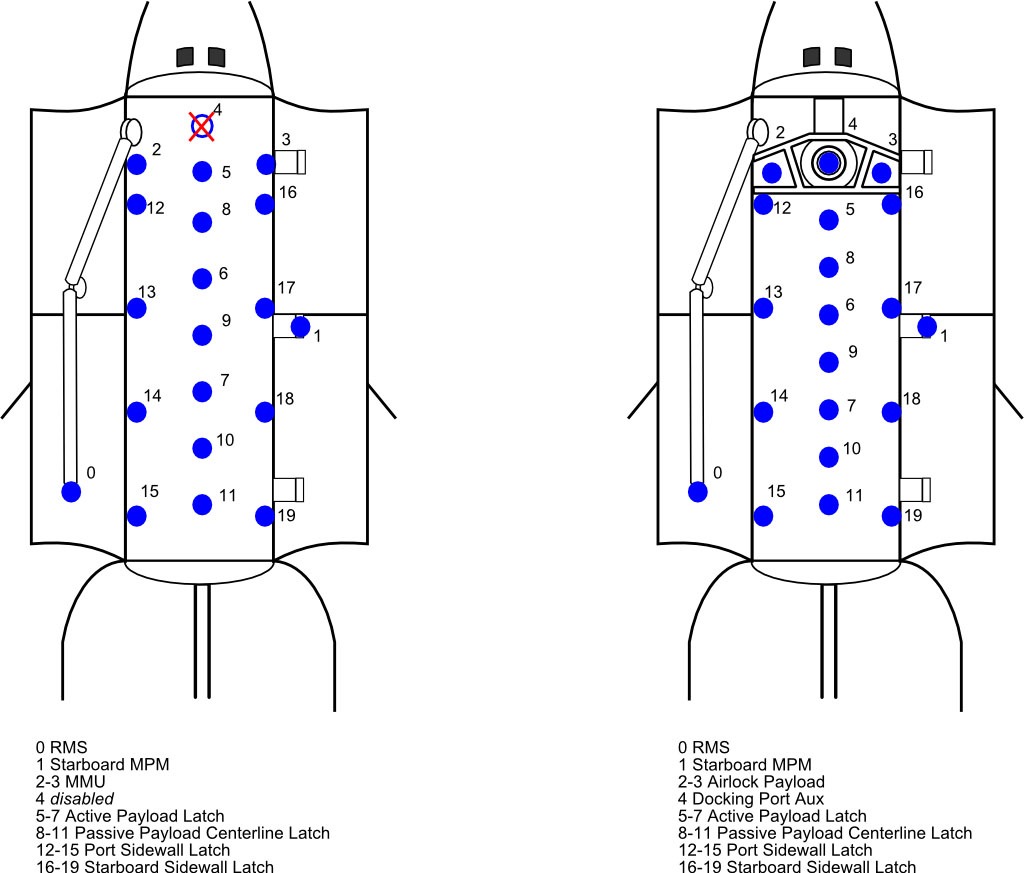
\includegraphics[width=1\textwidth]{SSU_Attachments.png}
  \caption{SSU attachment locations}
  \label{fig:SSUAttachments}
\end{figure}
\begin{multicols*}{2}
%\addcontentsline{toc}{subsection}{ Payload Operations Overview}
Payloads are attached through standard Orbiter attachment points. Figure \ref{fig:SSUAttachments} below will assist in visualizing the available attachment locations. The image on the left show the attachment locations without the ODS and the image on the rights shows the attachment locations with the ODS. Attachments 5 thru 11 are located just below the payload bay liner, so to have a correct vertical positioning of the payload, the attachment coordinates of the payload must be in its keel pin. Attachments 12 thru 19 are located on the side wall of the payload bay, just below the sill.\\
%Currently no payload bay bridgerails are shown; this makes payload berthing in the bay difficult.
If the payload is one that is deployed and later put back into the bay (example: MPLM), be sure to take note of the SRMS joint angles and orbiter XYZ coordinates displayed on panel A8U.
% For more information on the payload deploment and retreval systems see section 2.9.
The mission file entries to define the payload attachment positions are defined in Section \ref{sec:mission-files} of this manual.
The scenario file entries needed to add payloads to SSU are covered in Section \ref{sec:scenario-files} of this manual. \\

\newpage
%\begin{multicols*}{2}
\subsection{Extra Vehicular Activities and Docking Operations Overview}
Extra Vehicular Activity (EVA), or spacewalk, is used on some missions for work outside the shuttle, either for retrieving a satellite or most recently, for the assembly of the ISS. Independently of mission tasks, all missions have contingency EVA capability for manual payload bay door closure. EVA requires the use of an airlock, which on the shuttle can be located inside the middeck (Internal Airlock), or outside on the payload bay (External Airlock). EVA is currently not supported by SSU.\\
For missions requiring docking with the ISS or Mir, the orbiter need to be fitted with the Orbiter Docking System (ODS). The ODS is mounted on top of the External Airlock, and is controlled by buttons on panel A7L, allowing ODS powerup and docking ring extension and retraction.\\
\\
\WARNING{The next version of SSU will introduce changes to the docking port format. In addition to the docking port, there must exist an child attachment, in the same location, with the id ''APAS'' to achieve soft-docking. Without the attachment, docking will not be possible.}\\
\\
\\
For missions requiring the ODS to be located aft of its normal position (e.g. STS-88), the Tunnel Adapter Assembly (TAA) is positioned between the External Airlock and the forward bulkhead, effectively acting as a spacer. The TAA must also be used on missions carrying the Spacelab or the SpaceHAB modules. It must be placed at the forward end of the tunnel to provide a way in/out of the airlock during an EVA.\\
The mission file entries to define the ODS, External Airlock and TAA are defined in Section \ref{sec:mission-files} of this manual.
\end{multicols*}

\newpage
\subfile{SSU_SYSTEMS}
\newpage
\subfile{UPPER_STAGES}
\newpage
\subfile{FLIGHT_DATA_FILES}
\newpage
\subfile{MISSION_FILES}
\newpage
\subfile{SCENARIO_FILES}

\newpage
\section{CHANGE LOG}
\noindent
\textbf{Major changes from SSU 4.1}\\\\
$\rightarrow$ corrected issues with orbiter mesh\\
$\rightarrow$ added normal maps to OMS pods\\
$\rightarrow$ corrected MECO parameters of some missions\\
\\\\
\textbf{Major changes from SSU 3.0}\\\\
$\rightarrow$ corrected orbiter vehicle textures\\
$\rightarrow$ corrections to external airlock and tunnel adapter\\
$\rightarrow$ fixed orbiter vehicle mesh\\
$\rightarrow$ fixed Item 27 issue for OMS-2\\
$\rightarrow$ small corrections to RMS systems and its cameras\\
$\rightarrow$ corrected colors in displays\\
$\rightarrow$ added some functionality to Ku-band antenna (radar and manual slew)\\
$\rightarrow$ added Centaur upper stage and its vc panel\\
$\rightarrow$ added IUS upper stage and its vc panels\\
$\rightarrow$ updated HUD graphics\\
$\rightarrow$ fixed wrong WT parameter in MNVR display\\
$\rightarrow$ fixed issue with timer\\
$\rightarrow$ new texture for RMS\\
$\rightarrow$ fixed position of PLB handrails\\
$\rightarrow$ fixed reentry mesh not showing\\
$\rightarrow$ corrected the painting scheme on FWC SRBs\\
$\rightarrow$ corrected RMS and OBSS meshes\\
$\rightarrow$ new ET meshes\\


\newpage
\section{CREDITS}
Space Shuttle Ultra was originally based on Space Shuttle Deluxe. Large parts of the launch autopilot were copied (with minor modifications) from PEG MFD.
Some of the attitude control code was derived from Attitude MFD V3.
SSU also uses the KOST library.
SLC-6 uses part of VandenbergAFB-2006 by Usonian.\\
\\
This addon is open-source and is released under the GNU GPL. \\
\\
DISCLAIMER: The SSU team is not responsible for any crashes or other problems caused by this addon. Use at your own risk.
\end{document}